\section*{Problem 2 (10 pts)}

\newcommand{\bigCI}{\mathrel{\text{\scalebox{1.07}{$\perp\mkern-10mu\perp$}}}}
\begin{figure}[h]
    \centering
    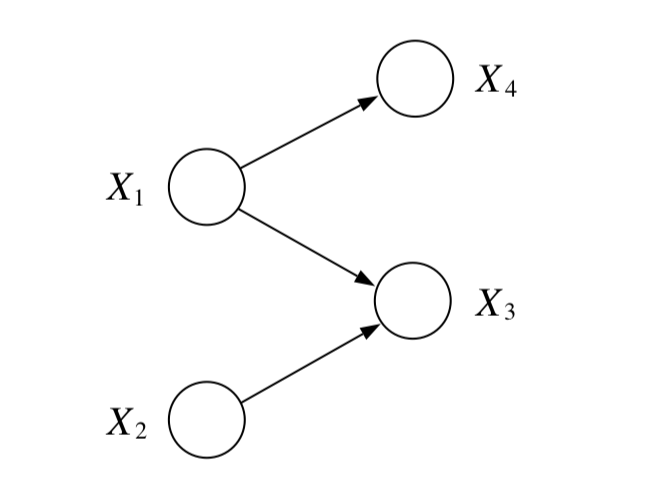
\includegraphics[scale=0.5]{images/written_2.png}
    \caption{Directed Graphical Model}
    \label{fig:my_label}
\end{figure}

\begin{enumerate}
    \item Without making any conditional independence assumption, given that each random variable can take $r$ values, how many parameters would be required to enumerate the joint distribution of the model in Figure~\ref{fig:my_label}? 
    You can start with writing down the joint distribution of the model as the product of the local conditional distributions shown in Figure~\ref{fig:my_label}. 

    \item State True or False for the following with required proof or reasons. 
    \begin{enumerate}
        \item \[  X_3 \bigCI X_4 \mid X_1 \]  
        \item \[  X_1 \bigCI X_2 \mid X_3 \] 
    \end{enumerate}
    
    \item Repeat part 2 assuming that the edges in the graph are undirected.
\end{enumerate}

\pagebreak

\begin{soln}{height=\textheight}
% Put your answer here.  Please make sure you complete your answers within the given size of the box.
\end{soln}